% Options for packages loaded elsewhere
\PassOptionsToPackage{unicode}{hyperref}
\PassOptionsToPackage{hyphens}{url}
\PassOptionsToPackage{dvipsnames,svgnames*,x11names*}{xcolor}
%
\documentclass[
  10pt,
  dvipsnames,enabledeprecatedfontcommands]{scrartcl}
\usepackage{amsmath,amssymb}
\usepackage{lmodern}
\usepackage{ifxetex,ifluatex}
\ifnum 0\ifxetex 1\fi\ifluatex 1\fi=0 % if pdftex
  \usepackage[T1]{fontenc}
  \usepackage[utf8]{inputenc}
  \usepackage{textcomp} % provide euro and other symbols
\else % if luatex or xetex
  \usepackage{unicode-math}
  \defaultfontfeatures{Scale=MatchLowercase}
  \defaultfontfeatures[\rmfamily]{Ligatures=TeX,Scale=1}
\fi
% Use upquote if available, for straight quotes in verbatim environments
\IfFileExists{upquote.sty}{\usepackage{upquote}}{}
\IfFileExists{microtype.sty}{% use microtype if available
  \usepackage[]{microtype}
  \UseMicrotypeSet[protrusion]{basicmath} % disable protrusion for tt fonts
}{}
\usepackage{xcolor}
\IfFileExists{xurl.sty}{\usepackage{xurl}}{} % add URL line breaks if available
\IfFileExists{bookmark.sty}{\usepackage{bookmark}}{\usepackage{hyperref}}
\hypersetup{
  colorlinks=true,
  linkcolor=Maroon,
  filecolor=Maroon,
  citecolor=Blue,
  urlcolor=blue,
  pdfcreator={LaTeX via pandoc}}
\urlstyle{same} % disable monospaced font for URLs
\usepackage{graphicx}
\makeatletter
\def\maxwidth{\ifdim\Gin@nat@width>\linewidth\linewidth\else\Gin@nat@width\fi}
\def\maxheight{\ifdim\Gin@nat@height>\textheight\textheight\else\Gin@nat@height\fi}
\makeatother
% Scale images if necessary, so that they will not overflow the page
% margins by default, and it is still possible to overwrite the defaults
% using explicit options in \includegraphics[width, height, ...]{}
\setkeys{Gin}{width=\maxwidth,height=\maxheight,keepaspectratio}
% Set default figure placement to htbp
\makeatletter
\def\fps@figure{htbp}
\makeatother
\setlength{\emergencystretch}{3em} % prevent overfull lines
\providecommand{\tightlist}{%
  \setlength{\itemsep}{0pt}\setlength{\parskip}{0pt}}
\setcounter{secnumdepth}{5}
%\documentclass{article}

% %packages
\usepackage{booktabs}
%\usepackage[left]{showlabels}
\usepackage{multirow}
\usepackage{multicol}
\usepackage{subcaption}

\usepackage{graphicx}
\usepackage{longtable}
\usepackage{ragged2e}
\usepackage{etex}
%\usepackage{yfonts}
\usepackage{marvosym}
\usepackage[notextcomp]{kpfonts}
\usepackage{nicefrac}
\newcommand*{\QED}{\hfill \footnotesize {\sc Q.e.d.}}
\usepackage{floatrow}

\usepackage[textsize=footnotesize]{todonotes}
\newcommand{\ali}[1]{\todo[color=gray!40]{\textbf{Alicja:} #1}}
\newcommand{\mar}[1]{\todo[color=blue!40]{#1}}
\newcommand{\raf}[1]{\todo[color=olive!40]{#1}}

%\linespread{1.5}
\newcommand{\indep}{\!\perp \!\!\! \perp\!}


\setlength{\parindent}{10pt}
\setlength{\parskip}{1pt}


%language
%\usepackage{times}
\usepackage{mathptmx}
\usepackage[scaled=0.86]{helvet}
\usepackage{t1enc}
%\usepackage[utf8x]{inputenc}
%\usepackage[polish]{babel}
%\usepackage{polski}




%AMS
\usepackage{amsfonts}
\usepackage{amssymb}
\usepackage{amsthm}
\usepackage{amsmath}
\usepackage{mathtools}

\usepackage{geometry}
 \geometry{a4paper,left=17mm, right = 17mm,top=25mm, bottom = 25mm}


%environments
\newtheorem{fact}{Fact}



%abbreviations
\newcommand{\ra}{\rangle}
\newcommand{\la}{\langle}
\newcommand{\n}{\neg}
\newcommand{\et}{\wedge}
\newcommand{\jt}{\rightarrow}
\newcommand{\ko}[1]{\forall  #1\,}
\newcommand{\ro}{\leftrightarrow}
\newcommand{\exi}[1]{\exists\, {_{#1}}}
\newcommand{\pr}[1]{\ensuremath{\mathsf{P}(#1)}}
\newcommand{\cost}{\mathsf{cost}}
\newcommand{\benefit}{\mathsf{benefit}}
\newcommand{\ut}{\mathsf{ut}}

\newcommand{\odds}{\mathsf{Odds}}
\newcommand{\ind}{\mathsf{Ind}}
\newcommand{\nf}[2]{\nicefrac{#1\,}{#2}}
\newcommand{\R}[1]{\texttt{#1}}
\newcommand{\prr}[1]{\mbox{$\mathtt{P}_{prior}(#1)$}}
\newcommand{\prp}[1]{\mbox{$\mathtt{P}_{posterior}(#1)$}}



\newtheorem{q}{\color{blue}Question}
\newtheorem{lemma}{Lemma}
\newtheorem{theorem}{Theorem}
\newtheorem{corollary}{Corollary}[fact]


%technical intermezzo
%---------------------

\newcommand{\intermezzoa}{
	\begin{minipage}[c]{13cm}
	\begin{center}\rule{10cm}{0.4pt}



	\tiny{\sc Optional Content Starts}
	
	\vspace{-1mm}
	
	\rule{10cm}{0.4pt}\end{center}
	\end{minipage}\nopagebreak 
	}


\newcommand{\intermezzob}{\nopagebreak 
	\begin{minipage}[c]{13cm}
	\begin{center}\rule{10cm}{0.4pt}

	\tiny{\sc Optional Content Ends}
	
	\vspace{-1mm}
	
	\rule{10cm}{0.4pt}\end{center}
	\end{minipage}
	}
	
	
%--------------------






















\newtheorem*{reply*}{Reply}
\usepackage{enumitem}
\newcommand{\question}[1]{\begin{enumerate}[resume,leftmargin=0cm,labelsep=0cm,align=left]
\item #1
\end{enumerate}}

\usepackage{float}

% \setbeamertemplate{blocks}[rounded][shadow=true]
% \setbeamertemplate{itemize items}[ball]
% \AtBeginPart{}
% \AtBeginSection{}
% \AtBeginSubsection{}
% \AtBeginSubsubsection{}
% \setlength{\emergencystretch}{0em}
% \setlength{\parskip}{0pt}






\usepackage[authoryear]{natbib}

%\bibliographystyle{apalike}



\usepackage{tikz}
\usetikzlibrary{positioning,shapes,arrows}

\ifluatex
  \usepackage{selnolig}  % disable illegal ligatures
\fi

\author{}
\date{\vspace{-2.5em}}

\begin{document}

\begin{center}

$\, $

\vspace{-10mm}

\textbf{\huge  Probability on Trial \linebreak \normalsize  Making Sense of Arguments and Stories}
\vspace{2mm}

Marcello Di Bello and Rafal Urbaniak
\end{center}

\hypertarget{the-book}{%
\section{The Book}\label{the-book}}

\vspace{-2mm}

\hypertarget{brief-description}{%
\subsection{Brief Description}\label{brief-description}}

\normalsize

``Probability on Trial'' is the first systematic philosophical defense
of legal probabilism, a research program whose aim is to harness the
powers of probability to analyze, model and improve the evaluation of
evidence and the process of decision-making in trial proceedings. The
book is informed by three questions. (1) Can the evidence presented at
trial be examined, weighed and assessed using probability theory? (2)
Can legal decision-making and standards of proof such as `proof beyond a
reasonable doubt' be defined using the language of probability? (3) Does
the deployment of probability theory in assessing evidence improve the
accuracy and fairness of trial decisions? We argue that the answer to
these questions is, by and large, affirmative.

Over the last fifty years, these questions have been debated in the
literature in philosophy, law, forensic science and artificial
intelligence. Despite considerable progress, legal probabilism faces
robust skepticism by legal scholars and philosophers. Many point out
that judges and jurors do not concern themselves with the probability
that the defendant is guilty, nor should they. It seems irresponsible,
even unjust, to decide about a person's life with numbers. Trials are
not gambles. Two rival theories hold prominence. The first is the
``story model'' (or its close cousin, ``relative plausibility'').
According to this theory, judges and jurors make sense of the evidence
presented at trial by constructing a unifying story or account of what
happened and how the evidence got there. The story that best explains
the evidence should prevail. Argumentation theory is another rival. It
emphasizes the fact that trials are adversarial. The arguments by one
side are scrutinized, attacked, challenged by the other side. The side
with the argument that resists all challenges should prevail. Both the
story model and argumentation theory provide important insights.
``Probability on Trial'' has a conciliatory and ecumenical aim. By
taking advantage of recent developments in artificial intelligence, in
particular Bayesian networks, it shows that probability theory can
factor in the insights from its rival theories and make them more
rigorous and precise. Hence, the subtitle reads ``Making Sense of
Arguments and Stories.''

This project is an exercise in philosophical imagination. What would
trial proceedings look like if probability played a more prominent role?
Would they be more accurate? Would they be more fair? We think they
would be, and we rely on a number of computer simulations written in
\textbf{\textsf{R}} to test this hypothesis. But even though the
argument is to a large extent revisionist of current trial practice, it
also pays close attention to it. The primary motivation for this project
comes from the unfortunate fact that the trial system makes mistakes.
Innocents are convicted. Perpetrators are acquitted. That this happens
is---we must admit, perhaps reluctantly---a reality. And certain racial
and socio-economic demographics tend to be disproportionately the
victims of mistaken trial decisions. How can the trial system best guard
against these errors and distribute them fairly when they occur? Many
have sought guidance in probability theory, the most well-developed
framework to tame uncertainty. ``Probability on Trial'' examines
whether, and if so how, probability can indeed be the right guide for
trial proceedings.

We wish to highlight the following contributions of the book:

\begin{itemize}
\item A probabilistic account, based on Bayesian networks, of concepts from the story model (coherence, completeness, specificity) and argumentation theory (rebutting, undercutting);
\item A solution to the problem of "unanticipated possibilities" via dynamic refinements of a Bayesian network or comparisons of multiple networks;
\item A response to standard philosophical objections leveled against legal probabilitm, particularly, the paradoxes of naked statistical evidence and the difficulty with conjunction; 
\item An account of the standard of proof in four criteria: high probability, coherence, resistance to objections, completeness);
\item A simulation-based argument that the tension between accuracy and fairness in trial proceedings is only apparent;
\item A comparison with other philosophical accounts of legal decision-making: the knowledge account, normic support, modal and causal accounts, relevant alternatives, comparative plausibility, foundherentism.
\end{itemize}

``Probability on Trial'' is aimed at philosophers with an interest in
legal epistemology and epistemology more generally. Many of the
difficulties of legal probabilism resemble difficulties faced by
Bayesianism in epistemology. The book will also be of interest to legal
scholars who have championed applications of probability theory to
evidence law as well as scholars who have resisted this trend. Another
target audience includes computer scientists and psychologists
interested in studying evidential reasoning and decision-making under
uncertainty. Besides contributing to the literature about legal
probabilism, the book aims to introduce unfamiliar readers to the rich
interdisciplinary debate on the topic, often scattered throughout
journals and books in philosophy, law, computer science, forensic
science and psychology. ``Probability on Trial'' can be a resource for
legal practitioners and reformers who aim to strengthen the protection
for defendants against wrongful convictions, improve the accuracy of
trial decisions and promote a fairer justice system. The audience is
broad: scholars, advanced undergraduates, practitioners and reformers.
Readers can follow different tracks through the book, depending on their
interests and inclinations. Some chapters present original research and
require technical background in probability theory. Others are
introductory, suitable for an advanced undergraduate course.

\hypertarget{outline}{%
\subsection{Outline}\label{outline}}

The book comprises five parts. Part I covers the current state of legal
probabilism and the challenges it faces. Part II describes the basic
formal tools, Bayes' theorem and the likelihood ratio, and their
limitations. Part III develops a more sophisticated theory using
Bayesian networks. Part IV turns to decisions and standards of proof.
Part V focuses on accuracy and fairness.

\vspace{2mm}

\noindent \textbf{Part I - Legal Probabilism and Its Foes}

\noindent The first part of the book will instill interest in legal
probabilism among unfamiliar readers and refresh seasoned readers about
the main points of contention. \textbf{Chapter 1} describes legal
probabilism in its infancy. In the early days, calculations were carried
out by hand. Bayes' theorem was used for weighing evidence and assigning
probabilities to hypotheses. Rules of decision were identified with
simple probability thresholds fixed via the maximization of expected
utility. This repertoire of ideas has proven useful in several ways,
especially in the assessment of explicitly quantitative evidence such as
DNA matches and expert testimony. At the same time, it has faced robust
opposition. \textbf{Chapter 2} describes the fierce scholarly debates
that accompanied the emergence of legal probabilism in the 20th century.
A host of conceptual difficulties emerged: the conjunction problem, the
problem of priors, and the paradoxes of naked statistical evidence.
These difficulties are well-known. Others are less familiar: the problem
of complexity, soft variables, unanticipated possibilities, and
corroboration.

The first two chapters provide the motivation for a deeper examination
of legal probabilism and the development of its more sophisticated
version. The remaining parts of the book cover two distinct topics:
evidence assessment (Part II and Part III, Chapters 3 through 10) and
decision-making (Part IV and Part V, Chapters 11 through 17). This
distinction reflects the fact that legal probabilism is both a theory of
evidence assessment (or evidence evaluation, evidence weighing) as well
as a theory of decision-making. These two topics are intertwined, but
are best kept separate for analytical clarity.

\vspace{3mm}

\noindent \textbf{Part II - Evidence Assessment First Pass}

\noindent The second part of the book discusses in great detail Bayes'
theorem and likelihood ratios, two formal tools essential for legal
probabilism. The objective is to understand how these tools help to
evaluate evidence and what their shortcomings may be.

\textbf{Chapter 3} begins with Bayes' theorem and surveys many of its
applications, for example, as a tool to avoid reasoning fallacies such
as the prosecutor's fallacy and the base rate fallacy. At the same time,
its applications are also limited. As discussed in \textbf{Chapter 4},
court cases often require fact-finders to weigh several pieces of
evidence, sometimes conflicting and susceptible to different
interpretations. The hypotheses that the fact-finders are asked to
evaluate in light of the evidence are structured stories or explanations
constituted by several sub-propositions. This level of complexity can
hardly be modeled by successive discrete applications of Bayes' theorem.
A more sophisticated machinery for evidence assessment is needed.

\textbf{Chapter 5} describes a formal tool distinct from Bayes' theorem
which many legal probabilists have found useful: the likelihood ratio.
Bayes' theorem requires one to assess the prior probabilities of the
hypothesis of interest. The problem is that assessing prior
probabilities is notoriously difficult. The likelihood ratio, instead,
offers a way to evaluate evidence without prior probabilities. We
illustrate how it can be used to evaluate both quantitative and
non-quantitative evidence, focusing in particular on DNA match evidence
and eyewitness testimony. Despite its versatility, however, the
likelihood ratio should be deployed with care. It can be hard to
interpret in practice and only provides a local assessment of the
evidence. A further problem, as critics have alleged, is that likelihood
ratios face difficulties in modeling the notion of evidential relevance
in certain cases.

Chapters 3 and 4 show that we need to move beyond simple legal
probabilism. Chapter 5 shows that likelihood ratios, while useful in
many ways, are still an unsatisfactory approach overall. The journey
toward a more sophisticated legal probabilism is accomplished in Part
III, Chapters 6 through 10.

\vspace{3mm}

\noindent \textbf{Part III - Evidence Assessment More and Better}

\noindent The third part of the book is motivated by two observations
about the evaluation of trial evidence. First, the process is holistic.
Judges and jurors make sense of the totality of the evidence not in a
piecemeal manner, but rather, by constructing a unifying narrative,
story or explanation. Many have criticized this story model because of
its potential for bias. Judges and jurors may discount important
evidence just because it does not fit with their preferred story.
Arguably, the best way to eliminate this worry is to deploy probability
theory and make the process of story construction more rigorous,
transparent and dependable. The second aspect of how evidence is
evaluated in trial proceedings is its adversarial structure. Each side
has the opportunity to scrutinize via cross-examination the evidence
presented by the other side. The defense may respond by attacking the
supporting evidence, the internal consistency of the prosecutor's
account, or by offering an alternative account.

Our working hypothesis is that Bayesian networks constitute the formal
machinery necessary for developing a more sophisticated legal
probabilism that is able to model these phenomena. The coherence of a
story as well as conflicts between pieces of evidence can be modeled by
corresponding properties of, operations on, and relations between
Bayesian networks.

\textbf{Chapter 6} offers a crash course on Bayesian networks with a
focus on the assessment of legal evidence. They are graph-like
structures that embody probability distributions and model complex
structures of evidence. A Bayesian network comprises a directed acyclic
graph (called a DAG) that represents relations of dependence between
variables, along with conditional probability tables corresponding to
these relations. In the last decade, the literature in artificial
intelligence and forensic science has made significant progress in
modeling holistic notions such as the coherence of a story and
argument-based notions such as conflicts between pieces of evidence. In
particular, Charlotte Vlek, together with Bart Verheij and Henry
Prakken, proposed to model the coherence of a story by adding a node in
the Bayesian network, call it a `story node.' The story node has other
nodes as its children corresponding to the events that make up the
story. In turn, these events are linked to their supporting evidence. An
example of a Bayesian network with a story node (or scenario node to use
Vlek's terminology) is depicted below:

\vspace{-2mm}

\begin{center}
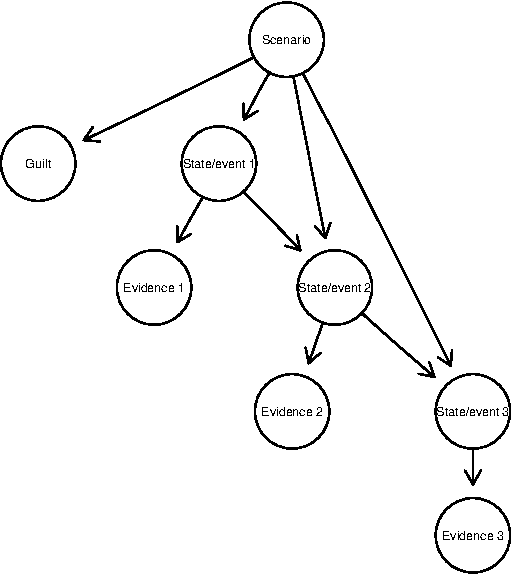
\includegraphics[width=8cm]{vlek-scenario-node.pdf}
 \end{center}

\vspace{-2mm}

\noindent Since the story node unifies the parts of a story, changes in
the probabilities of these parts can model the notion of coherence. The
stronger the (positive) probabilistic dependence between the different
parts, the more coherent the story. To model conflicts of evidence, a
Bayesian network can be built that comprises two competing stories, say,
one story put forward by the prosecution and another by the defense,
each supported by their own evidence. The network would specify that
these stories are incompatible and cannot be true concurrently. Another
approach to model conflicting evidence and competing stories was
developed by Norman Fenton and his research group. Separate stories are
represented by separate Bayesian networks, and Bayesian model comparison
is then used for assessing the comparative evidential support of the
competing stories.

\textbf{Chapter 7} assesses Vlek's story node approach as an account of
coherence. The critical argument is followed by a positive proposal.
Adding a story node by fiat---without any good reason for supposing that
the different parts of the story are connected other than being part of
one story---introduces unnecessary probabilistic dependencies between
the elements of a story. In addition, the story node approach is
simplistic as an account of coherence and fails to engage with the rich
philosophical literature on the topic. After the critical argument, the
chapter articulates a more adequate probabilistic account of coherence.
We define a formal notion of `story coherence' that reflects properties
of the Bayesian network used to model the evidence. We show that a
formal notion of `structured coherence' that reflect background causal
knowledge addresses the objections against probabilistic accounts of
coherence in the philosophical literature.

\textbf{Chapter 8} focuses on conflicts between pieces of evidence.
Neither Vlek's story node approach nor Fenton's model comparison
approach adequately capture how pieces of evidence and competing stories
may conflict with one another. The complex adversarial dialectic that
takes place in a trial cannot be modeled by simply averaging different
Bayesian networks (Fenton) or postulating relationships of
incompatibility between different story nodes (Vlek). We need an account
of more fine-grained notions, such as undercutting and rebutting
evidence, and more generally we need an account of how cross-examination
operates at trial. What cross-examination often accomplishes is not so
much the creation of an alternative story, but the reinterpretation of
an existing story by supplying additional information. We show that this
process of re-interpretation can be represented formally as the
refinement of an existing Bayesian network. Conflicts between pieces of
evidence such as undercutting and rebutting can be modeled by drawing
additional arrows between evidence nodes and hypothesis nodes.
Unanticipated possibilities and alternative scenarios that may arise in
the adversarial process can be modeled by comparisons across multiple
Bayesian networks.

The reverse of the phenomenon of conflicting evidence is that of
converging evidence, in particular, the fact that one piece of evidence
corroborates another. Corroboration has been the focus of extensive
scholarly debate often independently of the debates within legal
probabilism. \textbf{Chapter 9} surveys the literature on corroboration
and the main difficulties that have been leveled against proposed
probabilistic accounts. The chapter then formalizes a notion of
corroboration using Bayesian networks that overcomes most of the
difficulties of existing accounts.

Call the more sophisticated version of legal probabilism developed in
the chapters 6 through 9 legal probabilism 1.02. \textbf{Chapter 10}
draws some general morals by comparing legal probabilism 1.02 to other
accounts of judicial fact-finding, in particular, argumentation theory
and relative plausibility. Argumentation theory is well suited to model
conflicts between evidence, but cannot easily model the fact that
evidence may conflict more or less strongly with other evidence. Unlike
argumentation theory, legal probabilism 1.02 offers an account of
evidential support, conflict and convergence that captures how these
relations come in degrees of strength. The other competing theory we
consider, relative plausibility, is often criticized because the defense
need not present a full-fledged alternative story. Particularly in
criminal trials, it seems enough for the defense to weaken the
prosecutor's story and bring it below a threshold of acceptability.
Interestingly, legal probabilism 1.02 is flexible enough to model
competing stories (in agreement with relative plausibility) or model
conflicts without the need to construct a full-fledged alternative (as
critics of relative plausibility might prefer).

Legal probabilism 1.02 can still be challenged because of its
questionable empirical adequacy since judges and jurors hardly follow
probability theory. The claims of ``Probability on Trial'' are
theoretical and philosophical in nature. They rest on idealizations and
stylizations of the practice of trial proceedings. Nevertheless, we
emphasize how legal probabilism 1.02 offers a richer account of
evidential support beyond what critics have recognized. Susan Haack, for
example, criticized legal probabilism for its monodimensional account of
evidential support. This is true of simple legal probabilism in which
evidential support is modeled by the posterior probability of a
hypothesis given the evidence or the likelihood ratio. Legal probabilism
1.02, however, offers a richer account. In it, evidential support also
depends on the degree of specificity, completeness, and coherence of the
story put forward, and the extent to which the supporting evidence
withstands objections. These features can serve to formulate decision
criteria that are not unidimensional thresholds. Criteria for trial
decisions are discussed more extensively in the next part of the book.

\vspace{3mm}

\noindent \textbf{Part IV - Decision-making}

\noindent The third part of the book examines trial decision-making,
specifically, to what extent standards of proof such as `preponderance
of the evidence' and `proof beyond a reasonable doubt' can be understood
through the lenses of probability theory. There has been a spur of
research arguing that legal probabilism is unfit to model standards of
proof. But this research often holds a narrow view of legal probabilism.
We show that the version formulated in the previous chapters of the book
provides a more promising framework for theorizing about standards of
proof.

\textbf{Chapter 11} examines different strategies for theorizing about
standards of proof using probabilistic language. We begin with the most
natural decision criterion, a probability threhsold whose stringency is
determined by expected utility maximization. This account falls prey to
well-known objections, most notably, the puzzles of naked statistical
evidence and the difficulty with conjunction (discussed in greater
detail in later chapters). We then turn to alternative accounts, in
particular, the comparative strategy (Cheng) and the likelihood ratio
strategy (Dawid, Kaplow, Sullivan). Finally, we present our own
proposal. That is, the standard of proof is a function of several
criteria: the probability of liability, the specificity and coherence of
the accusatory story, the comprehensiveness of the supporting evidence
and its ability to withstand objections. We emphasize that these
criteria---probability, specificity, etc.---can be modeled using
Bayesian networks. So our proposal lies within the confines of legal
probabilism, though not the narrow version its critics have in mind. In
the following chapters, we illustrate the theoretical payoffs that come
from endorsing our proposal.

\textbf{Chapter 12} tackles the puzzles of naked statistical evidence.
This is a topic of enormous scholarly attention in the recent
philosophical literature. Our solution rests on two premises. First, an
accusation of liability should be substantiated by a well-specified
account---or story, narrative---whose moving parts are each supported by
adequate evidence. In cases of naked statistical evidence, the
probability of liability is high, but the specificity of the
accompanying narrative is suspiciously low. The second premise is that
the supporting evidence should typically be `causally grounded.' This
grounding contributes to a well-specified story and is achieved during
cross-examination by eliciting additional information about the relation
between the evidence and the alleged facts---for example, information
about the visibility conditions; the academic credential of an expert
witness; the chain of custody of a document. Interestingly, naked
statistical evidence blocks cross-examination because no undercutting
evidence can in principle be brought against it.

\textbf{Chapter 13} tackles another central problem for legal
probabilism, the difficulty with conjunction. We first provide a
detailed argument for why previous attempts in the literature on legal
probabilism have failed, focusing on the likelihood ratio approach by
Dawid and the comparative strategy by Cheng. Our proposal follows the
holistic approach by Allen and Pardo. We show how legal probabilism can
address the difficulty with conjunction so long as it can account for
holistic notions such as coherence and specificity. As noted already,
our working hypothesis is that the prosecution (or the plainitiff in a
civil trial) should aim to establish a well-specified accusatory
narrative whose moving parts are supported by adequate evidence. Once
the prosecution has accomplished that---and its case withstands
criticism---each element of the accusation is established to the
required standard if and only if the conjunction of these elements (that
is, the story as a whole) is established to the required standard.

\textbf{Chapter 14} compares our probabilistic account of
decision-making and standards of proof to other accounts in the
literature. We advance two main points of criticism. First, other
accounts are not necessarily incompatible with legal probabilism 1.02
which may in fact provide a more rigorous way to express their insights.
This point applies to foundeherentism (Hack), normic support (Smith),
argumentation theory (Sartor and Prakken) and to some extent relative
plausibility (Allen and Pardo). The second criticism we make is that
other accounts are engaged with what we might call `epistemology
fetishism'---that is, they borrow ideas in contemporary analytic
epistemology and force them onto legal-decision making. This criticism
applies in particular to knowledge accounts of legal proof. To be sure,
we might ourselves be accused of `probability fetishism'---that is,
unquestionably taking probability theory as a paradigm of rationality
and force it onto legal-decision making. Admittedly, there is no
empirical evidence that a probabilistic turn in legal decision-making
would improve trial decisions, if only because what it would mean to
`improve' trial decisions is unclear. A set of criteria are needed for
assessing the desired improvements. We tackle this normative question in
the final part of the book and show how probability theory can be of
service here.

\vspace{3mm}

\noindent \textbf{Part V - Accuracy and Fairness}

\noindent What values and objectives should trial decisions seek to
realize? What criteria and principles should guide trial decisions so
that they can further these values and objectives? The fourth part of
the book addresses these questions by focusing on improving the accuracy
and fairness of trial decisions.

As a preliminary step, \textbf{Chapter 15} surveys different values and
objectives that may inform the design of the trial system. In response
to criminal and civil wrongs, we assume that the state has, in
principle, the authority to impose punishments and decide about monetary
compensations. Given this assumption, we survey the most common values
and objectives that trial decisions should conform with: trial decisions
should be accurate; they should be fair; they should be accompanied by a
justification that is public and subject to scrutiny; they should be
reversible under appeal; they should contribute to further social
cohesion, compliance and deterrence; they should be humane and
respectful of people's dignity. We also explore to what extent these
values and objectives may be in tension with one another and to what
extent they can be subject to restrictions. The subsequent chapters
focus on two values and objectives: accuracy and fairness. We focus on
them, not because the others are not important, but because we believe
they are foundational for the others.

\textbf{Chapter 16} examines what it means for trial decisions to be
accurate and how accuracy can be promoted. There are different ways to
understand accuracy in trial decisions. We first distinguish accuracy in
the single instance and accuracy in the long run. Accuracy in the single
instance consists in the conviction of a defendant that is factually
guilty and the acquittal of a defendant that is factually innocent. A
similar definition applies to civil liability. Some have criticized the
notion of `factual guilt' on the ground that guilt is a judgment based
on evidence, not a state of affairs the exists objectively. We argue
that this view deprives trial decisions of objectivity and legitimacy.
We then turn to accuracy in the long run. In this sense, accuracy can be
understood as predictive or diagnostic. The former is the probability
that, if the defendant is found (not) liable at trial, the defendant is
actually (not) liable; the latter is the probability that if the
defendant is (not) liable, the defendant would (not) be found liable at
trial. The two notions are related but are not equivalent.
Distinguishing them has implications for how we should understand
standards of proof. To this end, we ask whether the standard of proof as
we defined in earlier chapters---consisting of multiple criteria such as
high probability of liability, narrative specificity and resistance to
objections----does in fact promote accuracy in the long run. We devise a
computer simulation that compares two models of the standard of proof.
On the first model, the standard of proof simply requires that the
defendant's liability be established with a high probability. On the
second model, the standard of proof requires, in addition to high
probability, that the narrative presented by the prosecution or the
plaintiff be reasonably specific. We compare the performance of the two
models. The first model prevails in terms of predictive accuracy, while
the second prevails in terms of diagnostic accuracy. We argue that
diagnostic accuracy, rather than predictive accuracy, is the most
adequate notion of accuracy for assessing trial decisions. We conclude
that understanding the standard of proof as the combination of a `high
probability' and `narrative specificity' (as we have argued in earlier
chapters) is a more rational model of the standard of proof.

\textbf{Chapter 17} turns to the fairness of trial decisions. What does
it means for trial decisions to be fair? In a formalistic sense,
fairness merely requires that every rule be applied to all defendants in
the same way. In a substantive sense, fairness requires, first, that
trial defendants not be subject to excessive burdens, and second, that
burdens (and benefits) be roughly equally distributed across different
defendants. Call the latter substantive comparative fairness. It can be
understood as the requirement that all defendants be exposed to roughly
the same risks of mistaken conviction. Equipped with this notion of
fairness, we examine whether admitting certain types of evidence makes
trial decisions unfair, and to what extent trial decisions are
inevitably unfair because of structural inequalities in society. We
argue that admitting certain forms of evidence, specifically profile
evidence and group-based generalizations, tends to burden certain groups
of defendants more heavily than others, thus deteriorating the fairness
of trial decisions. We also compare, via a computer simulation,
different models of the standard of proof and examine which model is
conducive to fairer trial decisions. We show that a standard of proof
that incorporates multiple criteria---such as high probability of
liability, specificity, resistance to objections and comprehensiveness
of the evidence---allocates burdens and benefits more fairly across
defendants than a standard of proof that simply requires that the
probability of liability be above a fixed threshold. Thus, the
multidimensional account of the standard of proof we have proposed fares
relatively well in light of normative criteria such as accuracy
(previous chapter) and fairness (this chapter).

\textbf{Chapter 18} draws some conclusions and points to open problems
for legal probabilism. We emphasize that our aim in the book is to show
that legal probabilism is a richer and more flexible theory that it
might seem at first. It is a theory that is able to incorporate insights
from other, possibly rival theories. Legal probabilism 1.02 can
satisfactorily address long-standing conceptual difficulties: the
problem of naked statistical evidence, the difficulty with conjunction,
corroboration and cross-examination. We also made some progress on other
conceptual difficulties, such as the problem of priors and the problem
of unanticipated possibilities. We underscore how, besides furthering
the academic debate, `Boosting Legal Probabilism' can be used by legal
practitioners and reformers who aim to strengthen the protection for
defendants against wrongful convictions, improve the accuracy of trial
decisions and promote a fairer criminal justice system. We sketch how
our theoretical findings can be implemented in the trial setting, but
leave a more precise articulation of the challenges of implementation
for future work.

\newpage

\vspace{-4mm}

\begin{center}\textbf{\large Table of contents}\end{center}
\begin{multicols}{2}
\footnotesize

\renewcommand{\labelenumi}{\Roman{enumi}}
\renewcommand{\labelenumii}{\arabic{enumii}}
\renewcommand{\labelenumiii}{\arabic{enumii}.\arabic{enumiii}}

\begin{enumerate}
\item Legal probabilism 1.01 and its foes
\begin{enumerate}

  \item The emergence of legal probabilism
  \begin{enumerate}
  \item  Famous cases
  \item  Probabilistic evidence
  \item  Trial by mathematics
  \item  Some history
  \end{enumerate}
  

  
  \item  A skeptical perspective
  \begin{enumerate}
  \item  The difficulty about conjunction
  \item  The problem of priors
  \item  Naked statistical evidence
  \item  The complexity problem
  \item  Soft variables
  \item  Corroboration
  \item  The reference class problem
  \item  Unanticipated possibilities
  \item  Non-probabilistic theories
  \end{enumerate}


\end{enumerate}
\item  Evidence assessment (first pass)


\begin{enumerate}


\setcounter{enumii}{2}
  \item  Bayes' theorem and the usual fallacies
  \begin{enumerate}
  \item  Assuming independence
  \item  The prosecutor's fallacy
  \item  Base rate fallacy
  \item  Defense attorney's fallacy
  \item  Uniqueness fallacy
  \item  Case studies
  \end{enumerate}

  
  
  \item  Complications and caveats
  \begin{enumerate}
  \item  Complex hypotheses and complex bodies of evidence
  \item Source, activity and offense level hypotheses
  \item  Where do the numbers come from?
  \item  Modeling corroboration
  \item  Stories, explanations and coherence
  \end{enumerate}

  
  \item  Likelihood ratios and relevance
  \begin{enumerate}
  \item Likelihood ratio as a measure of evidence strength
  \item The risk of false positive and its impact
  \item Hypothesis choice
  \item Levels of hypotheses and the two-stain problem
  \item Relevance and the small-town murder scenario
  \item The cold-hit confusion
  \item  Likelihood ratio and  cold-hit DNA matches
  \end{enumerate}


\end{enumerate}
\item  Evidence assessment (more and better)
\begin{enumerate}

\setcounter{enumii}{5}
\item  Bayesian Networks

  \begin{enumerate}
  \item  Bayesian networks to the rescue
  \item  Legal evidence idioms
  \item Scenario idioms
  \item Modeling relevance
  \item  Case study: Sally Clark
  \item DNA evidence
  \end{enumerate}
  
   \item Coherence
  \begin{enumerate}
  \item  Existing probabilistic coherence measures
  \item  An array of counterexamples
  \item Coherence of structured narrations with Bayesian networks
  \item  Application to legal cases
  \end{enumerate}
  
  
  \item Conflicts
  \begin{enumerate}
  \item Argumentation theory
  \item Undercutting and rebutting evidence
  \item Cross-examination
  \item Conflicting evidence in Bayesian networks
  \end{enumerate}
 
 
  \item Corroboration
  \begin{enumerate}
  \item Boole's formula and Cohen's challenge
  \item  Modeling substantial rise in case of agreement
  \item Ekel\"of's corroboration measure and evidentiary mechanisms
  \item General approach with multiple false stories and multiple witnesses
  \end{enumerate}


  \item  Towards legal probabilism 1.02
    \begin{enumerate}
    \item Outperforming competing accounts
    \item Empirical adequacy
    \item Specificity and coherence
    \item Resistance against objections 
    \item Comprehensive evidence
    \item Bayesian network implementation
    \end{enumerate}


\end{enumerate}
\item  Standards of proof
\begin{enumerate}


\setcounter{enumii}{10}
 \item  Are standards of proof thresholds?
  \begin{enumerate}
  \item  Legal background
  \item  Probabilistic thresholds
  \item  Theoretical challenges
  \item  The comparative strategy
  \item  The likelihood strategy
  \item  Probabilistic thresholds revised
  \item  Bayesian networks and probabilistic standard of proof
  \end{enumerate}


\item  Naked statistical evidence
  \begin{enumerate}
  \item  Forty years of hypothetical
  \item  Specific narratives
  \item  Cross-examination and causal grounding
  \item  Specificity, causality and Bayesian networks 
  \item  Are cold-hit DNA matches naked statistics?
  \end{enumerate}
  
  
\item  The Difficulty with Conjunction
  \begin{enumerate}
  \item  The problem
  \item  The likelihood strategy
  \item  The comparative stratgey
  \item  The holistic strategy
  \item  Complex bodies of evidence and structured narratives
  \end{enumerate}  

 \item  Other accounts 
  \begin{enumerate}
  \item  Baconian probability
  \item  Sensitivity
  \item  Normic Support
  \item  Foundherentism
  \item  Relevant alternatives
  \item  Knowledge
  \item  Relative Plausibility
  \item  Arguments
  \end{enumerate}

\end{enumerate}
\item  Accuracy and Fairness
\begin{enumerate}

\setcounter{enumii}{14}
  \item  The objectives of trial desicions
  \begin{enumerate}
  \item  Conceptual desiderata
  \item  Accurate and fair decisions
  \item  Protecting defendants
  \item  Public justification 
  \item  Revision and appeal
  \item  Dispute resolution and public deference
  \end{enumerate}




  \item  Accuracy and the risk of error
  \begin{enumerate}
  \item  Single case accuracy
  \item  Minimizing expected errors
  \item  Expected v.\ actual errors
  \item  Predictive and diagnostic accuracy
  \item  Error reduction and error distribution
  \item  Accuracy, high probability and specificity 
  \end{enumerate}


  \item  Fairness in trial decisions
  \begin{enumerate}
  \item  Procedural v.\ substantive fairness
  \item  Absolute v. comparative fairness 
  \item  Measures of fairness and measures of accuracy 
  \item  Profile evidence and group-generalizations
  \item  Structural inequalities 
  \item  A fairer standard of proof
  \end{enumerate}


\item Conclusions
\begin{enumerate}
\item  Assessing the progress made
\item  Open questions problems 
\item  To reformers and practitioners
\end{enumerate}
\end{enumerate}
\end{enumerate}

\end{multicols}

\normalsize

\hypertarget{outstanding-features-of-the-book}{%
\subsection{Outstanding Features of the
Book}\label{outstanding-features-of-the-book}}

\begin{itemize}
\item
  `Booosting Legal Probabilism' is the first comprehensive sustained
  philosophical examination of legal probabilism and how it fares
  against well-known objections. It is also conciliatory in admitting
  that many insights delivered by the critics of legal probabilism are
  valid and should be incorporated within the probabilistic approach to
  legal fact-finding.
\item
  The book is interdisciplinary. It closely engages with the literature
  in philosophy (see, for example, the discussion about coherence and
  corroboration) as well as literature outside philosophy, in artificial
  intelligence and in forensic science (see, for example, the discussion
  of Vlek's story node approach and Fenton's averaging).
\item
  The philosophical argument in defense of legal probabilism is
  accompanied by mathematical proofs as well as an \textbf{\textsf{R}}
  code implementation. This underscores the theoretical, practical and
  computational aspiration of `Boosting Legal Probabilism.'
\item
  The book is suitable for different audiences with different interests.
  It is partly introductory and partly describing original research by
  the authors. Instead of reading the entire book, one could follow
  different tracks. One could read the book to learn about the proof
  paradoxes (Chapter 2, 11, 12 and 13), Bayesian networks for evidence
  assessment and decision-making (Chapters 6 through 11, legal
  probabilism and its difficulties (Chapter 1, 2, 3, 4 and 11), the
  accuracy and fairness of trial decisions (Chapters 14, 16 and 17),
  etc. We will make sure to describe several tracks that readers could
  follow depending on their interests.
\item
  `Booosting Legal Probabilism' is divided into different parts, each
  tackling a distinct domain and level of analysis. The first half (Part
  II and Part III) examines how the evidence presented at trial should
  be assessed, weighed and evaluated using the tools of probability
  theory. The second half examines decisions at trial. The book offers a
  probability-based explication of legal standards of proof that is
  theoretically plausible (Part IV). In addition, the book also provides
  a normative justification of the proposed theory based on how
  standards of proof would perform in terms of accuracy and fairness
  under competing definitions (Part V).
\end{itemize}

\hypertarget{apparatus}{%
\subsection{Apparatus}\label{apparatus}}

\vspace{-2mm}

Besides the customary list of references at the end, the book will
contain multiple graphs and plots, Bayesian networks, and other data
visualizations generated via the \textbf{\textsf{R}} package
\texttt{ggplot2} as is standard in publications in statistics and
machine learning.

Since computer simulations play an integral part in the argument, the
book will be accompanied by supplementary materials available on-line.
These materials will contain the \textbf{\textsf{R}} source code for the
simulations along with tutorials for readers interested in learning the
technical details. Some of the derivations and results will be also
supported by associated \textbf{\textsf{Mathematica}} notebooks, which
will also be made freely available.

\hypertarget{competition}{%
\subsection{Competition}\label{competition}}

\normalsize

Several books in print cover topics at the intersection of evidence, law
and probability. They, however, do not have the same aims as our book,
and since they can be sensibly grouped with respect to how our book will
differ from them, we'll discuss them in batches accordingly.

\todo{double check if all references have publishers}

\begin{itemize}

\item Consider first the key books written by legal theories and philosophers, such as 
Stein (2005), \textit{Foundations of Evidence Law}, Oxford University Press; Ho (2008), \textit{A Philosophy of Evidence Law: Justice in the Search for Truth}, Oxford University Press; Haack (2014), \textit{Evidence Matters: Science, Proof, and Truth in the Law}, Cambridge University Press; Nance (2016), \textit{The Burdens of Proof: Discriminatory Power, Weight of Evidence, and Tenacity of Belief}, Cambridge University Press;    Dahlman, Stein, and Tuzet (eds.) (2021), \textit{Philosophical Foundations of Evidence Law}, Oxford University Press.
These books offer original theories of evidence law, the standards of proof and legal decision-making  under uncertainty.   They address, from a philosophical perspective, many of the conceptual difficulties that we examine in our book. But they do not develop a probabilistic theory of evidence and decision-making that crucially relies on Bayesian networks.  Nor do they combine analytic arguments, mathematical proofs and computer simulations.  They also focus on rather abstract examples and their use of real-life cases and discussions between the practitioners is rather limited.

\item  Many books by forensic scientists and computer scientists  have championed applications of Bayesian networks to legal evidence evaluation, for example, Taroni, Aitken, Garbolino and Biedermann (2006) \textit{Bayesian Networks and Probabilistic Inference in Forensic Science}, Wiley;   Taroni,  Bozza,  Biedermann, Garbolino and  Aitken (2010), \textit{Data Analysis in Forensic Science: A Bayesian Decision Perspective}, Wiley; Fenton and Neil (2012/2018) \textit{Risk Assessment and Decision Analysis with Bayesian Networks}, Chapman and Hall/CRC Press. These books are groundbreaking in that they offer a detailed examination of how expert evidence can be assessed using Bayesian networks. They, however, do not address philosophical problems such as the problem of naked statistical evidence or the difficulty of conjunction, nor do they aim to offer a novel theory of the standard of proof, and they make no connection to the  narrative approach or evidence evaluation criteria brought up by the critics of legal probabilism. Unlike our book, they do not address normative questions such as the accuracy or fairness of trial decisions.

\item Several books exists about Bayesian networks that are more general in content. Some of them focus on the technical dimension,  such as Scutari and  Denis (2014), \textit{Bayesian Networks With Examples in R}, (Neapolitan 2004), \emph{Learning Bayesian Networks} or Fenton, Neli and Martin (2013), \emph{Risk Assessment and Decision Analysis with Bayesian Networks}. Some are more psychological and use Bayesian networks to examine how our minds rely on evidence to understand the world and solve problems, such as Spirtes, Glymour and Scheines (2000), \emph{Causation, Prediction and Search}, Glymour (2001),  \emph{The mind's arrows. Bayes Nets and Graphical Causal Models in Psychology}, or Lagnado (2021), \textit{Explaining the Evidence: How the Mond Investigates the World}, Cambridge University Press. \todo{More needs to be said about Lagnado, as he does focus on legal evidence} These general books  lack  focus on legal applications (some legal applications are discussed in Fenton, but the coverage is fairly narrow as compared to our intent---the authors focus on covering on presenting a few technical representation methods of various types of evidence). 



\item There are books that focus exclusively on the evaluation of statistical and probabilistic evidence at trial. They include Robertson and Vignaux (1995), \textit{Interpreting Evidence: Evaluating Forensic Science in the Courtroom}, Wiley [second edition:  Robertson, Vignaux and Berger, published in 2016];  Lucy (2005), \textit{Introduction to Statistics for Forensic Scientists}, Wiley;  Finkelstein (2010), \textit{Statistics for Lawyers}, Springer; Balding and Steele (2015), \textit{Weight-of-Evidence for Forensic DNA Profiles}, Wiley;  Buckleton, Bright and Taylor (eds.) (2016) \textit{Forensic DNA Evidence Interpretation}, CRC Press. These books differ from our own because they are more specific, often focusing on just  DNA evidence or select forms of expert evidence. Besides DNA and expert evidence, our book also covers common forms of evidence, such as eyewitness testimony. In addition, these books are written from the perspective of forensic science and do not examine the   philosophical issues that are in the focus in our book, and they do not develop a general approach to the probabilistic modelling of narrations.

\item  Finally, a few books focus on the legal and ethical problems that arise from relying on statistical and actuarial evidence at trial and in the criminal justice system more generally. These books include Schauer (2006), \textit{Profiles, Probabilities and Stereotypes}, Belknap Press; Harcourt (2008), \textit{Against Prediction: Profiling, Policing, and Punishing in an Actuarial Age}, University of Chicago Press. Some chapters of our book discuss  actuarial and statistical evidence, but this is not our sole focus. In addition, the authors of these books do not rely on legal probabilism as their guiding theoretical framework.


\end{itemize}

\hypertarget{market-considerations}{%
\section{Market Considerations}\label{market-considerations}}

\hypertarget{the-primary-market}{%
\subsection{The Primary Market}\label{the-primary-market}}

\normalsize

The target audience comprises scholars in various disciplines, primarily
philosophers and legal theorists with an interest in epistemology,
evidence and decision-making under uncertainty. Computer scientists and
psychologists who work on similar topics will also be interested in
reading the book.

Selection of chapters from the book are suitable to be used as primary
readings in advanced undergraduate courses or graduate seminars with
titles such as Legal Probabilism, Legal Epistemology, Probability and
the Law, Bayesian Epistemology, Bayesian Networks in Philosophy,
Statistics in the Law, Math on Trial. We have ourselves taught similar
courses in the past and felt the need of a book such as ours. We believe
other instructors felt the same.

\hypertarget{status-of-the-work}{%
\section{Status of the Work}\label{status-of-the-work}}

We plan 16 chapters, two of which already exist, so 14 remain. We
predict each chapter will take around 2 months to complete, which
results in 28 months of work. We add eight months for proofreading,
delays, revisions and running various versions of the chapters by our
colleagues, so overall the fairly lenient schedule suggests completion
after three years.

With appendices the existing chapters have around 32k words each. We
expect the early chapters chapters (including appendices) to be shorter,
and the later chapters to be of approximately that length, the whole
book being around 350k words.

It is not clear how many graphs will be needed. Early chapters won't
need many, the existing chapters have around 10-15 each (including
appendices). Supposing this is the number for eight chapters, we seem to
be looking at 80-100 graphs and visualizations.

We have already used some of the materials on which this book is based
in graduate seminars, for example, in the seminar Bayesian Networks in
the Philosophy that one of us taught at Arizona State in Spring 2021. We
plan to use select chapters to teach graduate seminars and advanced
undergraduate courses. By the time the book is published, we hope to
have student-tested a significant portion of the book (in compliance
with copyright restrictions as needed).

To better reach our intended audience, we plan to present portions of
the book at international conferences in the coming years. We have been
invited to an international conference in Girona, Spain on Evidence Law
in Spring 2022. This conference gathers some of the leading scholars in
law, philosophy, forensic science and psychology interested in topics at
the intersection of law, evidence, probability and decision-making.

We do not plan to include any material requiring additional copywright
permissions.

\hypertarget{sample-chapters}{%
\section{Sample Chapters}\label{sample-chapters}}

Two sample chapters with their appendices are attached to this
submission.

\hypertarget{reviews}{%
\section{Reviews}\label{reviews}}

\begin{itemize}

\item Floris Bex

\item Alex Biedermann

\item Edward Cheng

\item Christian Dahlman

\item Norman Fenton

\item David Lagnado

\item Anne Hsu

\item Brian Hedden

\item Silja Renooij

\item Frederick Schauer

\item Silvia Bozza

\item Bart Verheij



\end{itemize}

\hypertarget{author-background}{%
\section{Author Background}\label{author-background}}

Two CVs are attached to this submission.

\end{document}
